\chapter{Experiment Proposal}
\label{chapter:metricExperiments}
In the previous chapters, we have discussed algorithms related to the algorithm ranking problem. We are able to rank algorithms based on distance and evaluate the quality of such ranking. As was discussed in Sections \ref{section:distanceBasedRanking} and \ref{section:rankingQuality}, we can easily plug distance based ranking into the quality evaluator. The remaining argument missing is to provide $IDatasetDistance$ interface. We have discussed several algorithms being able to conform to this interface. Some of these algorithms need extra information as an input -- weights. This enables us to optimize the weights in order to maximize the quality of ranking.
We begin by defining the \emph{optimization problem} in which some space of parameters is searched in order to get the optimal solution given some evaluation criteria. We then introduce the class of optimization algorithms called \emph{Genetic Algorithms} (GAs) that are inspired by the evolution of species occurring in the nature. The general form of the algorithms is outlined and different parts are discussed -- \emph{selection}, \emph{crossover} and \emph{mutation} in more details.

We can use the GAs to optimize the weights of the algorithms for measuring the dataset distance. Metadata available was discussed in the previous chapter. 
Several experiments are proposed on the data available. Baseline, attribute alignment, and global attribute distance measure based on weighted $p$-norm with different values of $p$ explored and weights optimized by the evolution. Further, attribute assignment with the attribute distance measure  based on weighted $p$-norm with different values of $p$ tried and weights optimized by the evolution. Final experiment proposed in this section is the aggregation of the global and attribute distance measures with the importance of both counterparts also optimized. 

A big picture of all algorithms plugged together is provided. This will be possible because we have been careful in proposing algorithms in such a way that algorithms are easily pluggable to others, as they conform to the same interfaces. This overview is useful, as the number of algorithms plugged in together is large, and the whole workflow is complicated.
We also discuss the choice of all other settings of all algorithms (extending attribute space by $\dummy$ attributes, parameters for the GA, etc.)
The parameters will be chosen according to the results of Theorems \ref{theorem:metricPreservation}, \ref{theorem:dummyConstantMinimalDistance}, and \ref{theorem:metricRestoration}, so the resulting distance between datasets is a metric.
We will review the results of our experiments and discuss them. As we will see, new proposed algorithms can outperform the baseline and even improve the global attribute distance with statistical significance.

\section{Optimization}
We have provided a means of measuring the quality of distance based ranking. Some of the distances are based on weighted $p$-norms. We could try to find out such weights that result in the best ranking according to the evaluator. This is captured by the following definition:
\begin{definition}
	In the \emph{optimization problem} we have an \emph{objective function} $f$ over a domain (or search space) $A$: $f: A \rightarrow \mathbb{R}$. In the case of a \emph{minimization} problem, the solution is $x \in A$ such that $\forall y \in A: f(x) \le f(y)$. The \emph{maximization} solution is $x \in A$ such that $\forall y \in A: f(x) \ge f(y)$.
\end{definition}
In some cases, it may be hard to find the solution of the optimization problem. Some algorithms do not guarantee the optimal solution and returns its approximation instead.
\section{Genetic Algorithms}
\label{section:geneticAlgorithms}
\emph{Genetic algorithm} is a meta search heuristic based on Charles Darwin’s evolution theory \cite{Darwin} and the laws of inheritance inferred from Gregor Mendel’s inheritance theory \cite{Mendel1866}. According to the evolution theory, the following facts hold:
\begin{itemize}
	\item Every species is fertile enough that if all offspring survived to reproduce the population would grow.
	\item Despite periodic fluctuations, populations remain roughly the same size.
	\item Resources such as food are limited and are relatively stable over time.
	\item Individuals in a population vary significantly from one another, and much of this variation is inheritable.
\end{itemize}
From these assumptions, the theory infers the following:
\begin{itemize}
	\item A struggle for survival ensues.
	\item Individuals less suited to the environment are less likely to survive and less likely to reproduce; individuals more suited to the environment are more likely to survive and more likely to reproduce, and leave their inheritable traits to future generations, which produces the process of natural selection.
	\item This slowly effected process results in populations changing to adapt to their environments, and ultimately, these variations accumulate over time to form new species.
\end{itemize}
According to the inheritance theory, inherent properties of each organism are encoded in a structure called genotype. Genotype consists of genes. Each gene corresponds to some trait in organism (e.g. colour of eyes). Genotype is inferred from parents’ genotype by crossing over their genetic material. Genotype may be also altered during organism lifetime by mutation. A phenotype is the composite of an organism's observable characteristics or traits, such as its morphology, development, biochemical or physiological properties, phenology, behaviour, and products of behaviour. Relationship between genotype and phenotype is often conceptualized as follows:

\begin{equation*}
genotype + environment \rightarrow phenotype.
\end{equation*}

Genetic algorithms (GA) were described by Holland \cite{HollandGeneticAlgorithms}, who utilized principles of the evolution and inheritance theory. Given an optimization problem, GA views the solution to the problem as an individual. In the original John Holland’s work, the individual was binary encoded, but other encodings are suitable as well. The algorithm can also treat genotype equal as phenotype and the individual directly maps to the solution. In other situation, phenotype can be derived from the individual either deterministically or stochastically. Example of the former would be treating negative values of the individual as positive or encoding of the neural network, the example of the latter would be creating an individual according to the grammar described in the genotype with different rules applicable at the same time. 

A number of individuals form a population. At first, a population of individuals is created (either randomly or by using some known sub-optimal solutions). Individuals are then evaluated based on their ability to solve the problem by a function known as fitness. Individuals proceed to next generation with probability proportional to their fitness (this step is known as \emph{selection}). In each generation, new individuals are created from random parents in the current population (this step is known as \emph{crossover}) and some individuals in the current population are altered (this step is known as \emph{mutation}). New generations continue to be created until a termination criterion is satisfied (usually conditions on fitness of some individual, average fitness in population, number of generations or time elapsed since the start of the algorithm). A pseudocode of simple genetic algorithm is shown in Algorithm \ref{algo:geneticAlgorithm}.

\IncMargin{1em}
\begin{algorithm}
	\SetKwInOut{Input}{input}
	\tcp{Pseudocode of the main loop of the genetic algorithm.}
	\BlankLine
	$P_0 \leftarrow$ initialize-population()\;
	$t \leftarrow 1$\;
	\While{\upshape termination-criterion not satisfied}{
		$P_{t+1} \leftarrow$ selection$(P_t)$\;
		crossover$(P_{t+1})$\;
		mutation$(P_{t+1})$\;
		$t \leftarrow t+1$\;
	}
	\Return bestIndividual($P_t$)\;
	\caption{Genetic Algorithm}\label{algo:geneticAlgorithm}
\end{algorithm}\DecMargin{1em}

Since genetic algorithms are stochastic and do not guarantee finding an optimal solution, it could be sometimes beneficial to repeat the whole process and take the best individual from all runs.
Mutation, crossover and other steps altering the population are often generalized as genetic operators. Genetic operators will be described when applied to one or several individuals; expansion of the operators on the whole population is typically done by applying the operator on each individual or on a sample of individuals from the population.

\subsection{Selection}
Selection determines how many offspring the individuals will have in the next generation. This should be based on fitness - in general, fitter individuals should have more offspring than those less fit. Common approaches to the selection are:
\begin{itemize}
	\item \emph{Roulette selection} – let $f_k$ be a fitness of an individual $k$. Let $F_s$ be the sum of the fitness of all individuals ($F_s = \sum_{i=1}^{n}f_i$, where $n$ is the population size). For each position in the next generation, the roulette is spun. In each spin an individual is selected with probability $\cfrac{f_k}{F_s}$.
	\item \emph{Scaling} – same as the roulette selection, except that fitness is scaled at the beginning. The most common scaling function is linear function. This can solve some problems in case all individuals have similar fitness (more like random walk) or when there are very large fitness gaps between individuals (high pressure on selecting best individuals).
	\item \emph{Rank based} – individuals are sorted by fitness in ascending order. Probability of selection is higher with higher index in the sorted set of individuals.
	\item \emph{Tournament selection} – for each position in next generation, a tournament of $n$ individuals is held. The best individual is selected by the tournament with some fixed probability $p$. If the best individual is not selected, the second best individual is selected with probability $p$ and so on. If all previous individuals are not selected, select the worst individual from the tournament. This rescales the population and thus the evolution pressure remains constant (extraordinary good individuals does not flood entire population and even the minor differences between individuals are recognized).
\end{itemize}

Some alternations of GAs perform the selection not only among the new offspring, but also among parents. Furthermore, the best solution found so far may be lost during the process. To counter this, the best individuals are sometimes guaranteed to be inserted into the next generation. This is referred to as \emph{elitism}.

In binary coding, crossover is typically implemented as a one point crossover – two parents are selected, then one point in both parents is chosen randomly, and the parts induced by the point chosen are swapped. This creates two offspring individuals. A more general alternative is the $n$-point crossover, where more points are chosen when creating the offspring. One point crossover is illustrated in Figure \ref{fig:crossover}.

\begin{figure}
	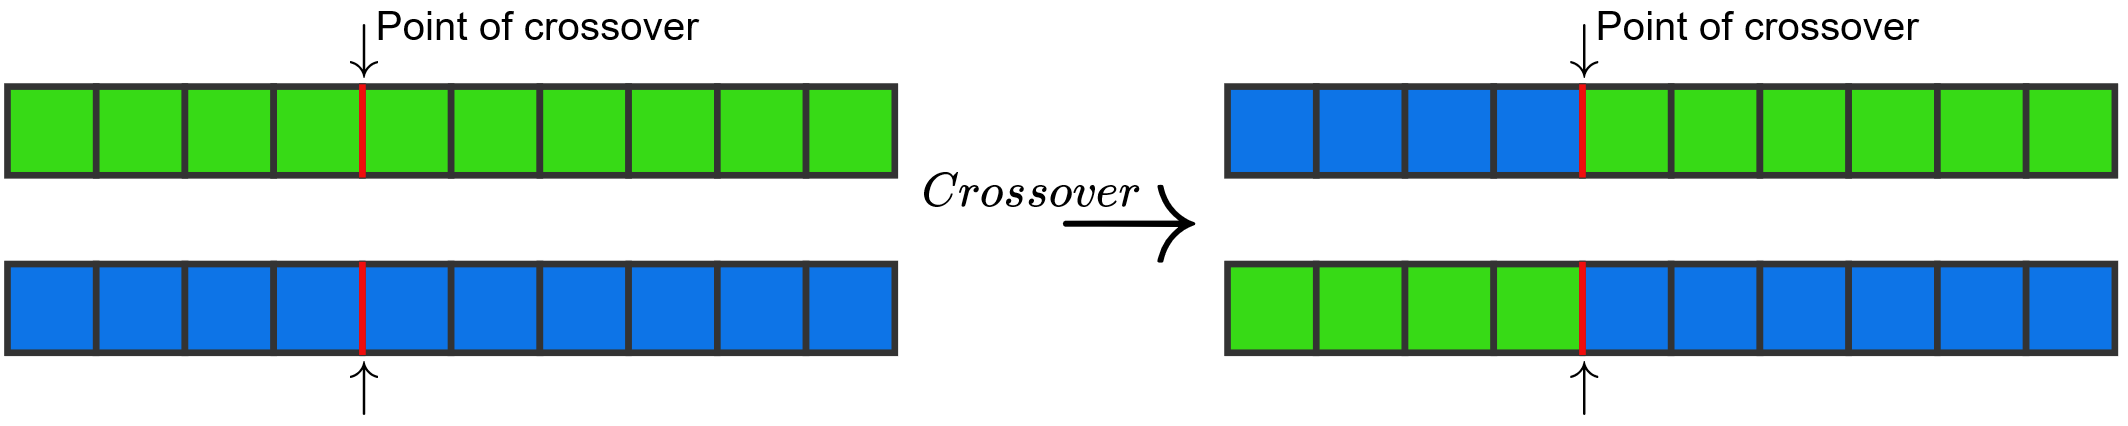
\includegraphics[width=14cm]{Images/crossover.png}
	\centering
	\caption{Example of the crossover genetic operator.}
	\label{fig:crossover}	
\end{figure}

\subsection{Mutation}
Mutation operator alters a part of an individual, thus introducing new features into population. Mutation helps explore those parts of the search space that would be otherwise hard to reach with selection and crossover only. In particular, mutation helps the genetic algorithm get out of the local optima.
In binary coding, mutation is typically implemented in a way that each bit has some small probability $p_{mutation}$ of being flipped. This is illustrated in Figure \ref{fig:mutation}.

\begin{figure}
	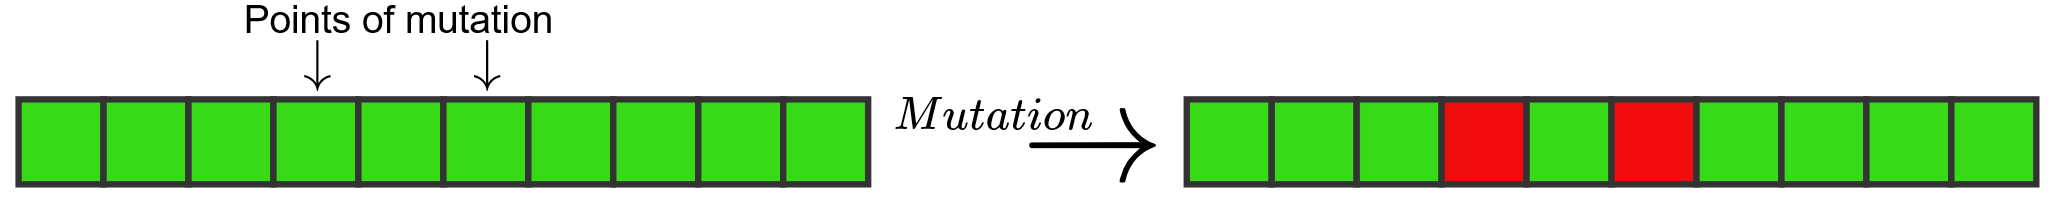
\includegraphics[width=14cm]{Images/mutation.png}
	\centering
	\caption{Example of the mutation genetic operator.}
	\label{fig:mutation}	
\end{figure}

\subsection{Modifications}
One of the advantages of genetic algorithms is their versatility. It is easy to change different parts of the algorithm to accustom for the needs.
For example if we have some knowledge about the problem we aim to solve, we may introduce operators tailored to the problem. Such operators often achieve better results than classic non-specialized operators.
Alternatively, we can create additional evolutionary pressure if the evaluation of the fitness is costly (either time or money) so the algorithm converges quickly. Other approaches include controlling the parameters, so the algorithm does not get stuck in local optima and the diversity of individuals in the population is empowered.

\section{Experiments}
\label{section:firstExperiments}
We have all the pieces we need to propose different experiments settings. We have different ranking measures, different distances measures that can be optimized, optimization algorithm, data, metadata, and we are also able to evaluate the quality of different ranking algorithms. In this chapter, we finally connect these components together.
Since we have designed the system interfaces in a versatile way, we will be able to plug in different components into algorithms, thus changing the behaviour in a certain way. This will enable us to use the same framework for evaluation although the settings used may be totally different.

When proposing the full framework for experiments, we will use the top-down approach. This is because the algorithm on the top will be either the same or will not change so often and will be providing the unified experiment framework. The experiment part will be mainly carried in the bottom of the framework where we will be trying different settings and combination. The rest of this section is dedicated to the description of our experiments.

The goal of the experiments is to find a good settings for solving the ranking problem. We will use the OpenML dump discussed in Chapter \ref{chapter:obtainingData} as the data source. The quality of settings will be verified by the Ranking Quality Assessment algorithm (Algorithm \ref{algo:rankingQualityEvaluation}). The Ranking Quality Assessment needs an implementation of $IRanking$ interface as an input. According to the discussion in Section~\ref{section:baseline}, the baseline algorithm is useful in order to verify that the extra complexity present in different models has indeed improved the ranking quality. Therefore, as the first setting to try, we will add the baseline algorithm built by Algorithm \ref{algo:rankingBaseline}. This algorithm does not need any additional information other then data, thus we are finished with this experiment branch. Different implementation of $IRanking$ interface discussed in the thesis were distance based rankings. One suitable algorithm was $k$-NN algorithm (Algorithm \ref{algo:k-nnRanking}).

 Other distance based algorithms were also discussed but we were inclined to use the simpler algorithm, as the whole framework is quite large and we did not want to add an extra layer of logic or complexity without a specific reason. The transformation of $IDistanceRanking$ to $IRanking$ is done by the $partial$ application as described in Algorithm \ref{algorithm:IDatasetRankingTransformarmation}. The $k$-NN algorithm needs, besides data, a parameter $k$ and a notion of distance between datasets, as captured by the $IDatasetDistance$ interface (Algorithm \ref{interface:IDatasetDistance}). As discussed in Section~\ref{section:openMLDump}, the size of the neighbourhood should be set high enough so it is probable that the neighbourhood will contain all algorithms. We have set the $k$ to 17 (10 percent of the training datasets).

Throughout the thesis, we have discussed many options how to implement the $IDatasetDistance$. In this chapter, our aim will be to set up all the algorithms conforming to the $IDatasetDistance$ interface so the resulting distance is a metric. We will explore the non-metric settings in the chapters to follow. In Section \ref{section:distanceUsingGlobalMetadata} we reviewed distance based on global attributes. As we have shown, any distance defined on global metafeatures based on the weighted $p$-norm is a metric. The corresponding $IDatasetDistance$ implementation was outlined in the Global Metadata Distance algorithm (Algorithm \ref{algo:globalMetadataDistance}). We will try the most common types of $p$-norms -- that is $1$-norm, $2$-norm and $\infty$-norm. We let the Genetic Algorithm optimize the weights of the $p$-norms. The settings and the genetics operators used for optimizing the weights will be discussed later. 

Other implementations of the $IDatasetDistance$ interface were proposed in Chapter \ref{chapter:attributeAssignment}. These algorithms were able to deal with the unstructured dataset space by attribute assignment. We will discuss them starting with the simpler ones. Algorithm \ref{algo:attributeAlignmentMasterThesis} needs just the mapping of attribute into a single number -- $\sigma$. We have decided to use selectors for this approach. Concrete mapping for attributes were number of categories in the case of categorical attributes and difference between maximum and minimum in the case of the numerical attributes. We could also try different attribute evaluation functions $\sigma$ but regarding the time complexity to conduct the experiments, we decided to focus computational power on more expressive languages. Furthermore, Algorithm \ref{algo:attributeAlignmentMasterThesis} is a special case of Algorithm \ref{algo:combinedAlignmentHungarian}, and it is sufficient to try the more generic version to asses the potential of attribute assignment techniques. Other attribute assignment algorithms were Attribute Assignment algorithm (Algorithm \ref{algo:attributeAlignmentHungarian}) and the more generalised version the Combined Attribute Assignment algorithm (Algorithm \ref{algo:combinedAlignmentHungarian}) that split the assignments into multiple assignments given by the selectors. 

As discussed in Section \ref{section:distanceUsingAttributes}, we found it more sensible to calculate assignments of numerical and categorical attributes separately and not to mix numerical and categorical attributes together. The latter would limit the number of metafeatures that could be used. Furthermore, we argued that the distance between a categorical and a numerical attribute should be naturally high -- possibly reached by the penalization for addition of the $\dummy$ attributes to each selector. We thus decided not to use the Attribute Assignment algorithm but rather to use its more generic version -- Algorithm \ref{algo:combinedAlignmentHungarian}. We used two selectors -- one selecting categorical attributes and the other selecting the numerical attributes (Algorithms \ref{algo:CategoricalAttributesSelector} and \ref{algo:NumericalAttributesSelector}). According to Corollary \ref{corollary:metricPreservation}, the Combined Attribute Assignment algorithm produces a metric if the attribute distance measures of corresponding selectors are metric on the attribute space. According to this, we have to define categorical and numerical attribute distance as a metric. Again, we will use the most common weighted $p$-norms -- $1$-norm, $2$-norm and $\infty$-norm.  We shall set the $p$ of the norm in the same manner and we will not try one value of $p$ for the categorical distance and a different value for the numerical distance. However, we let weights to be set independently (also, the number of metafeatures is different). We will also optimize the weight of each assignment result. Again, we will use Genetic Algorithm for the optimization with the settings discussed later. Finally, we will carry out experiments with the aggregation of global and attribute metafeatures (Algorithm \ref{algo:datasetDistanceCombination} -- Dataset Distance Aggregation). We will use Algorithms \ref{algo:globalMetadataDistance} and \ref{algo:combinedAlignmentHungarian} as sub-distances. The selectors used will be the same as in the rest of the experiments. Again, we will use the same value of $p$ for each algorithm and selector. We let GA optimize all weights occurring in the algorithm including weight of each sub-distance.

We have prepared a cluster of computers to conduct the experiments with various hardware and operating system. The system was composed of MySQL database for storing the results, local SQLite database with metadata and experiment results that were distributed together with the application. As this database was large and was needed to be retrieved before each experiment, we decided to add to the application to reduce network load with multiple runs and to allow for faster queries to the database. The experiments run on the Microsoft .Net platform using C\# programming language. This is a platform that is currently supported by Windows, although there is .Net runtime called Mono for Unix-like system that has limited capability compared to the whole framework. However, we made sure to use the part of .Net that can be run by Mono, therefore we could use all the major OS platform - Windows, Unix and Mac OS. To allow for really easy redistribution, the Docker Image \cite{docker} was created. Docker is an open-source project that automates the deployment of applications inside software containers, by providing an additional layer of abstraction and automation of operating-system-level virtualization on Linux. This means that every docker image should be deployable to every computer that has docker installed. The image also has all the requirements installed like installed shared libraries and packages. This allows for smooth running of the experiments just by running the image. The image is automatically downloaded form the docker repository after entering the run command.

Before we discuss the concrete settings for the experiments, we would like to recapitulate the complexities of the whole workflow and underlying algorithms. 

If the ranking is precomputed, the computation of ranking quality has a complexity of $\mathcal{O}(n_dn_a)$ where $n_d$ is the number of datasets and $n_a$ is the number of algorithms.
 The complexity of ranking is constant for the baseline (whereas building up the baseline function takes  $\mathcal{O}(n_dn_a + n_a\log(n_a))$ time). For the distance based ranking, the $k$-NN algorithm takes $\mathcal{O}(n_d\log(n_d)+n_a\log(n_a))$ time per dataset, provided we have a distance matrix precomputed. This results in $\mathcal{O}(n_d(n_d\log(n_d)+n_a\log(n_a)))$ steps for all datasets. We will conduct the distance computation outside to save time as discussed in Section \ref{section:distanceBasedRanking}. To compute the distance between every pair of dataset we need $\mathcal{O}(n_d^2c(\globalDistance))$, where c$(\globalDistance)$ is the cost of computing the distance $\globalDistance$ between some pair of datasets. The complexity of computing the distance $\globalDistance$ using the global metadata for some parameter $p$ is $\mathcal{O}(n_m),$ where $n_m$ is the size of the vector of global metadata. The missing complexity is computing $\globalDistance$ using the assignment techniques. The selectors we use merely check whether attribute is numerical or categorical, therefore the complexity of each selector is $\mathcal{O}(n_{att})$. 
 
 The Attribute Alignment (Algorithm \ref{algo:attributeAlignmentMasterThesis}) in our case has the complexity of $\mathcal{O}(n_{att}\log(n_{att})),$ where $n_{att}$ is the bound of number of attributes in datasets (given by the selector). This is because computing the evaluation function $\sigma$ is easy if the $\sigma$ represents number of categories or difference between maximum and minimum. The complexity of Attribute Assignment with selectors (Algorithm \ref{algo:combinedAlignmentHungarian}) is $\mathcal{O}(c(\attributeDistance)n_{att}^2+ n_{att}^3)$, where $c(\attributeDistance)$ is the cost of attribute distance function. In our case the $c(\attributeDistance)$ is $\mathcal{O}(n_{att\_met})$ -- the size of the vector of attribute metadata. The $c(\attributeDistance)n_{att}^2$ part is for computing the distance matrix between two sets of attributes and the rest is for the Hungarian method. Finally, the complexity of Dataset Distance Aggregation (Algorithm \ref{algo:datasetDistanceCombination}) is the sum of complexities of individual sub-distances.
 
 The exact values of different variables influencing the complexities are shown in Table \ref{table:complexityVariablesValues}. 
 \begin{table}[htbp]
 	\caption{Values of variables influencing the complexity given by the training data.}
 	\label{table:complexityVariablesValues}
 	\centering
 	\begin{tabular}{ |c | c | c | }
 		\hline
 		Variable & Description & Value \\
 		\hline                       
 		$n_d$ & Number of attributes &  170\\
 		$n_a$ & Number of algorithms &  115 \\
 		$n_m$ & Number of global metafeatures &  31 \\
 		$n_{att}$ & Bound of number of attributes& 50   \\
 		$n_{att\_met}$ & Number of attribute metafeatures & 47    \\
 		\hline  
 	\end{tabular}
 \end{table} 
 
 The total complexity for the whole workflow for different setups of the ranking algorithms are in Table \ref{table:totalComplexities}.
 
 \begin{table} 
 	\caption{Total complexity of the whole workflow for ranking quality evaluation for different ranking algorithms.}
 	\label{table:totalComplexities}
 	\centering 
 	\renewcommand{\arraystretch}{1.3}
 	\begin{tabular}{|c| c| c|}
 		\hline %inserts horizontal line
 		Algorithm & Total Complexity (in $\mathcal{O}$) & Optimizing \\
 		\hline 
 		Baseline & $n_dn_a + n_dn_a + n_a\log(n_a)$ & No\\ 
 		\hline 
 		Attribute Alignment& $\begin{array} {r@{}l@{}} & {} n_dn_a + n_d(n_d\log(n_d)+n_a\log(n_a)) \\ & {} + n_d^2n_{att}\log(n_{att}) \end{array}$ & No\\    \hline 
	 	Global Distance& $\begin{array} {r@{}l@{}} & {} n_dn_a + n_d(n_d\log(n_d)+n_a\log(n_a)) \\ & {} + n_d^2n_m \end{array}$ & Yes\\    \hline 
 		Attribute Assignment& $\begin{array} {r@{}l@{}} & {} n_dn_a + n_d(n_d\log(n_d)+n_a\log(n_a)) \\ & {} + n_d^2(n_{att\_met}n_{att}^2+n_{att}^3) \end{array}$ & Yes\\    \hline 
 		Aggregation& $\begin{array} {r@{}l@{}} & {} n_dn_a + n_d(n_d\log(n_d)+n_a\log(n_a)) \\ & {} +  n_d^2(n_{att\_met}n_{att}^2+n_{att}^3+n_m) \end{array}$ & Yes\\    \hline 
 	\end{tabular}
 \end{table}
 
 
 
When optimizing the weights of either attribute distance or dataset distance, the complexity provided is the complexity to evaluate one individual. It is interesting that given one weight, we have to evaluate the weighted $p$-norm $\mathcal{O}(n_d^2(n_{att}^2)$ times to build up a distance matrix. As the weights are all that compose the individual in this case, we can look at our task as a reinforcement learning task, as we get a feedback from environment after $\mathcal{O}(n_d^2(n_{att\_met}n_{att}^2))$ steps.

Apparently, workflows including attribute assignments are the most costly ones. Just expression $n_d^2(n_{att\_met}n_{att}^2+n_{att}^3)$ in our case is equal to $170^2(47+50^2+50^3) \approx 2*170^250^3=7,225,000, 000$. Note that this is not the exact amount of steps taken as the expression is in $\mathcal{O}$, it merely gives the idea about the complexity of the workflow for our data. 
It takes up to three days to compute the ranking quality of the Attribute Assignment algorithm optimized by evolution with 100 individuals and 100 generations on the Intel I7 computer with sufficient amount of memory. This was a value that had to be taken into account when proposing the settings for assignment algorithms.

In algorithms with attribute assignments, the decision about how to extend attribute space with $\dummy$ has to me made. We did not want to penalize too heavily for having different number of attributes. As we want to have a metric and such small penalization is not possible for artificial $\dummyoutside$ attributes by Theorem \ref{theorem:dummyConstantMinimalDistance}, we decided to use $\dummyinside$ attribute from the attribute space. Based on the same argument with small penalizations, we created $\dummyinside$ attribute that has the value of every metafeature equal to the median value of all values of that metafeature in both the training and testing set.

The settings for the evolution was set according to our previous experiments and few short preliminary experiments we performed to estimate good values. We were not able to tune the parameters because of the computation times mentioned above. We decided to use tournament selection with elitism to preserve the best values. The tournament probability of better individual winning was set to 60 percent and the tournament size was set to three. This was to discourage earlier convergence and to boost the generalization ability. We have used crossover with the probability of 75 percent and the mutation with the probability of 10 percent. Population size was set to 100 in order to have reasonably big population and still be able to finish the computation in reasonable time. The number of generation was set as a termination criterion. The exact value was set to 70. This was again chosen based on the time of computation, while allowing for some sufficient amount of evolution cycles to evolve interesting properties. Furthermore, we did not want to have too many generations so the algorithm does not have a big opportunity to overfit the found solutions. The weights were randomly initialized out of $\langle 0,1 \rangle$ uniform distribution. However some operators could push the weight values outside of this interval -- even to zero or negative values. According to Theorem \ref{theorem:weightedpnormisnorm}, the weights must be strictly positive to have a metric. Therefore we use genotype to phenotype mapping by using the absolute value of the weights. We still allow weights to be zero. This would break the coincidence metric axiom but we rather interpret it as the algorithm decided that the corresponding metafeature is a noise, and therefore the attribute space should not contain this metafeature.

\begin{figure}	
	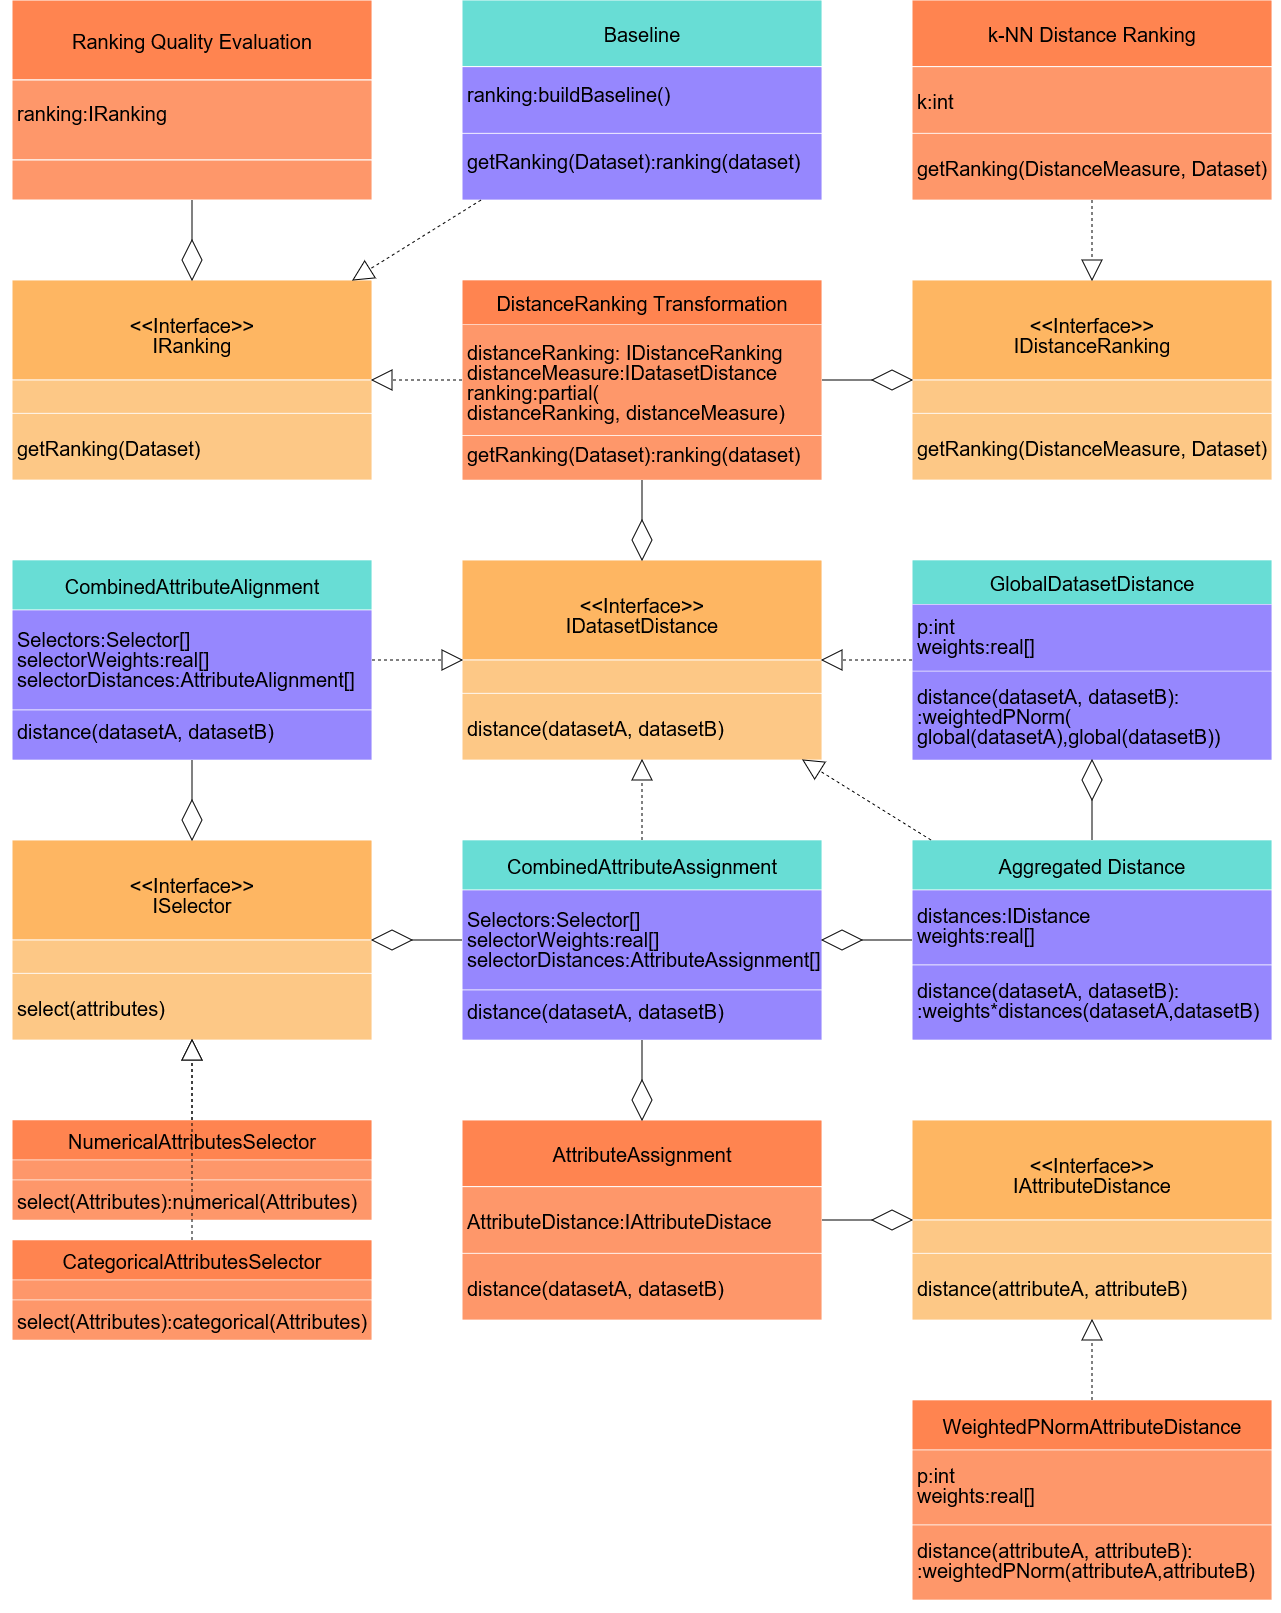
\includegraphics[width=15cm]{Images/BigPictureMetrics.png}
	\centering
	\caption{UML diagram of the whole workflow. Violet rectangles represent different ranking algorithms that will be tried in the experiments. Global Dataset Distance, Combined Attribute Assignment and Dataset Distance Aggregation will have their weights optimized by the genetic algorithm. The fitness will be provided by the Ranking Quality Evaluation. }	
	\label{fig:BigPictureMetrics}	
\end{figure}

\subsection{Results}
The results of experiments proposed in this chapter are described in the following paragraphs. Our framework uses Algorithm \ref{algo:rankingQualityEvaluation} to measure average Spearman's rank correlation coefficient (Equation \ref{eq:averageSpearman}) on the training and testing data. The higher value the better, whereas value 1 is a theoretical maximum, value -1 is a theoretical minimum, and value 0 is as good as a random guessing.

The baseline scored 0.551659 on the training set and 0.540807 on the testing set. Attribute Alignment algorithm had both testing and training score below 0.5. We believe this was because we did not optimize this algorithm. We will not discuss this algorithm further, as it is a special version of the Attribute Assignment algorithm.

The raw results of all metric-producing experiments on the testing set can be seen in Table \ref{table:metricResults}. As the runs did not have any order by definition, we sorted the values so that the first run of every algorithm corresponds to the best result of that algorithm and so on.

\begin{table}[ht]		
	\centering
	\caption{Evaluation of ranking quality of metric algorithms on the testing dataset.}
	\label{table:metricResults}	
	\begin{tabular}{cllll}

		\toprule
		\multirow{2}{*}{Run} & \multicolumn{3}{c}{ $p = 1$} \\
		\cmidrule{2-4} & Global & Assignment & Aggregation \\
		\midrule		
		1 & 0.556977 & 0.5495 & 0.563649 \\
		2 & 0.556756 & 0.54561 & 0.563345 \\
		3 & 0.556341 & 0.545248 & 0.563046 \\ 
		4 & 0.556282 & 0.543699 & 0.56146 \\
		5 & 0.555896 & 0.542449 & 0.560571\\
		6 & 0.55554 & 0.540697 & 0.559257\\
		7 & 0.555343 & 0.540422 & 0.558868\\
		8 & 0.555299 & 0.540328 & 0.558767\\
		9 & 0.555105 & 0.54024 & 0.556617\\
		10 &  0.554622 & 0.53886 &	0.556128\\
		Median & 0.555718 & 0.541573 & 0.559914 \\
		\midrule
		\multirow{2}{*}{Run} & \multicolumn{3}{c}{ $p=2$} \\
		\cmidrule{2-4} & Global & Assignment & Aggregation \\
		\midrule
			1 & 0.554876 & 0.553777 & 0.563032	\\
			2 & 0.554851 & 0.547558 & 0.560352 \\
			3 & 0.554324 & 0.547426 & 0.560273 \\ 
			4 & 0.554175 & 0.547255 & 0.558913\\
			5 & 0.554089 & 0.54587 & 0.55852\\
			6 & 0.553832 & 0.544282 & 0.557389\\
			7 & 0.553628 & 0.543237 & 0.556919\\
			8 & 0.553458 & 0.543211 & 0.556625\\
			9 & 0.553423 & 0.542909 & 0.556509\\
			10 & 0.553093 & 0.542443 & 0.554418\\
			Median &0.553961 & 0.545076 & 0.557955 \\
			\midrule
			\multirow{2}{*}{Run} & \multicolumn{3}{c}{ $p=\infty$} \\
			\cmidrule{2-4} & Global & Assignment & Aggregation \\
			\midrule
			1 & 0.557636 & 0.549426 & 0.560815	 \\
			2 &	0.55736 & 0.546354 & 0.560662 \\
			3 &	0.557084 & 0.544777 & 0.556537 \\ 
			4 &	0.557026 & 0.544307 & 0.552372 \\
			5 &	0.556069 & 0.543048 & 0.551713 \\
			6 &	0.55585 & 0.542675 & 0.551215 \\
			7 &	0.555551 & 0.541701 & 0.55055 \\
			8 &	0.555429 & 0.540912 & 0.550265 \\
			9 &	0.555058 & 0.540544 & 0.545764 \\
			10& 0.554629 & 0.537932 & 0.545444 \\
			Median &0.555959 & 0.542861 & 0.551464 \\
		\bottomrule
	\end{tabular}
\end{table}
From the raw results it can be seen that some algorithms are better than others. From the point of view of the median of the results, the order of algorithms is as follows (from best to worst): (Aggregation with $p=1$), (Aggregation with $p=2$), (Global with $p$=$\infty$), (Global with $p=1$), (Global with $p=2$), (Aggregation with $p=\infty$), (Assignment with $p=2$), (Assignment with $p=\infty$), (Assignment with $p=1$), baseline.
 
 To have a proper comparison, results of each algorithm on the testing set were compared based on the result of two tailed \emph{Mann-Whitney U Test} \cite{manWhitney}. This test is a non-parametric test with the null hypothesis that both samples come from the same population. The $\alpha$ statistics used was 0.05. The results of the tests are in Table \ref{table:metricComparisonStatisticalSignificance}. All algorithms except the Assignment algorithm with the $p=1$ were significantly better than the baseline. The best results had the aggregation of assignment and global metadata. There was no algorithm that would be significantly better than any of the Aggregated algorithms. On the contrary, Aggregated algorithms with $p=1$ and $p=2$ were significantly better than every other algorithm. There was no clear winner between those two. The results proof our hypothesis that algorithms based on attribute assignment produce useful results for ranking prediction. Also, our theory that the best results are probably obtainable by the aggregation of assignment and global distance is also supported by the results. Interesting observation is that the assignment with $p=1$ produces the worst results but the aggregation with the same $p$ provides the best results. Perhaps alignment with $p=1$ provide best additional information to support decision by the global metadata.
 
 \begin{table}[ht]		
 	\centering
 	\caption{Statistical comparison of different algorithms and their ranking quality results on the testing set. Row $i$ defines what algorithms had significantly worse results than algorithm $i$. N stands for no and Y for yes. }
 	\label{table:metricComparisonStatisticalSignificance}	
\begin{tabular}{r|cccccccccc}
	&
	\rot{Aggregation, $p=1$} &
	\rot{Aggregation, $p=2$} &
	\rot{Global, $p=\inf$} &
	\rot{Global, $p=1$} &
	\rot{Global, $p=2$} &
	\rot{Aggregation, $p=\infty$} &
	\rot{Assignment, $p=2$} &
	\rot{Assignment, $p=\infty$} &
	\rot{Assignment, $p=1$} &
	\rot{Baseline}

	
	\\ \hline
	Aggregation, $p=1$        &   & N & Y & Y&Y &Y &Y &Y &Y & Y  \\ 
	Aggregation, $p=2$        &   & & Y & Y& Y& Y& Y& Y&Y & Y  \\ 
	Global, $p=\infty$       &   & &  &N & Y & N & Y & Y & Y & Y  \\ 
	Global, $p=1$        &   & &  & & Y & N & Y & Y & Y & Y  \\  
	Global, $p=2$        &   & &  & &  & N & Y & Y & Y & Y  \\  
	Aggregation, $p=\infty$    &   & &  & &  & & Y & Y & Y & Y  \\  
	Assignment, $p=2$     &   & &  & & & & &N & N& Y  \\ 
	Assignment, $p=\infty$   &   & &  & & & & & & N& Y  \\ 
	Assignment, $p=1$     &   & &  & & & & & & & N  \\ 
	 \hline
\end{tabular} 
\end{table}


The best results on the testing set were produced by the aggregation of global and attribute metafeatures where the $p$ was set to 1. The evolution progress is shown together with the baseline in Figure \ref{fig:bestTrainingCombined}. We have measured evaluation score of the currently best individual only for statistics purpose and such measurement did not influence the run of the algorithm. It is however useful to see whether some overfitting occurred. As can be seen, the baseline was surpassed after the first generation on the training set and was above the testing baseline at all times. We can also see very high correlation between the improvement on the training set with the improvement on the testing set. At some points, some decrease of performance on the testing set can be seen but is compensated for in the further generations.
 
\begin{figure}	
	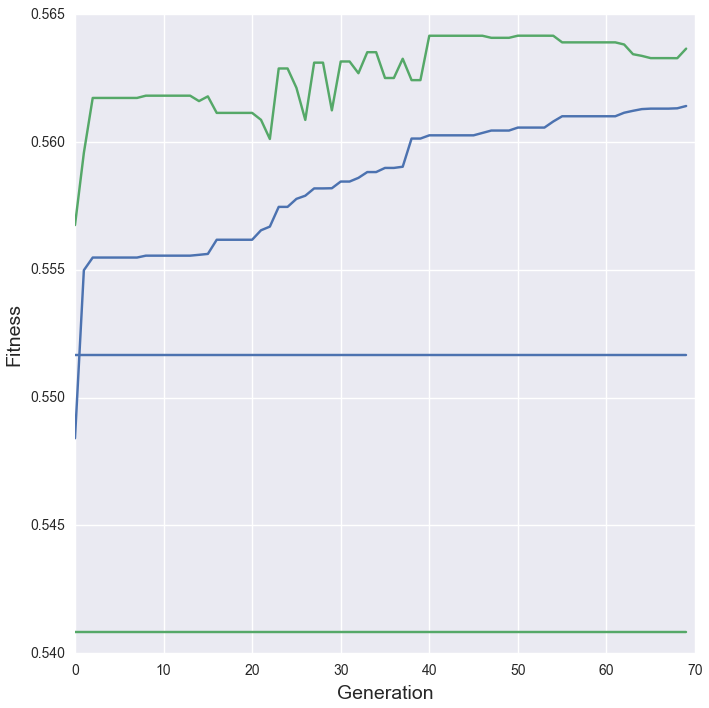
\includegraphics[width=14cm]{Images/bestTrainingCombined.png}
	\centering
	\caption{Evolution progress of the individual with the best result on the testing set together with the baseline. Results on the training set are blue, on the testing set are green. On the $x$-scale is the evolution progress, on the $y$-scale is the quality of ranking measured by the Spearman's correlation coefficient.}	
	\label{fig:bestTrainingCombined}	
\end{figure} 
 
 \subsection{Visualisation of the Distance}
 The visualization can be important for humans to interpret the results. This can be possible using kernel methods described in Section \ref{section:kernels}. Using kernelized PCA, we can project the space into two dimensions, which can be easily visualized. This requires inner product kernel. However, algorithms we use are producing metrics instead of kernels. There is a connection between these two concepts as metric represents dissimilarities and kernels similarities. We can transform distance to similarity by subtracting the distance from some large enough constant. This may not be an inner product kernel, however lots of kernel methods perform well enough with similarities close to inner products \cite{DistancesAndIndefiniteKernelsForTheSetsOfObjects}. Other approach is to repair the resulting similarity by one of the techniques proposed in \cite{PDKernels}. We have used kernelized PCA by taking the distance evolved during the run of aggregation of global and attribute approach with the best result on the testing set. The distance to similarity was transformed as follows:
 $$\text{similarity}(x,y)=100 - \Delta(x,y).$$
 The visualization of the training set is depicted in Figure \ref{fig:kpcaDistance}. We can see few clusters, but the space is mostly well covered. To check the plausibility of the visualization, we investigated the cluster of datasets in the top right region defined by $x$-component $> 1.3$ and $y$-component $> 0.2$. The datasets are listed in Table \ref{table:visualizationCluster} together with several selected metafeatures. Every dataset in the cluster is a binary classification tasks with very similar Default Accuracy. Therefore, the visualization seems to be plausible.
Being able to visualize the data is important, as it allows for a much easier interpretation.
 
 \begin{table}[ht]		
 	\centering
 	\caption{Datasets in one of the clusters in the visualization of the distance (Figure \ref{fig:kpcaDistance}).}
 	\label{table:visualizationCluster}	
 	\begin{tabular}{cccccc}
 		
 		\toprule
 		Name & OpenMLId & Attributes & Classes & DefaultAccuracy & Rows \\
 		\midrule		
 		fri\_c0\_250\_5 & 776 & 6  & 2  &  0.5 & 250 \\
 		fri\_c3\_250\_5 & 744 & 6  &  2 &  0.564 & 250	\\
 		no2 & 886 & 8  & 2  &  0.502 & 500 \\
 		wind & 847 & 15  & 2 &  0.532552  & 6574 \\
 		pbc & 810 & 19  & 2 &  0.550239  & 418 \\
 		analcatdata\_apnea3 & 764 & 4 & 2 & 0.535715 & 450 \\
 		\bottomrule
 	\end{tabular}
 \end{table}
 
 % \begin{definition}
% 	A real symmetric $N \times N$ matrix K is called  positive definite if its associated quadratic form is positive for any nonzero coefficient vector $c=[c_1, \dots, c_N]^T \in \mathbb{R}^N$, i.e.,
% 	\begin{equation}
% 	\sum_{i=1}^{N}\sum_{j=1}^{N}c_ic_jK_{ij}>0.
% 	\end{equation}
% \end{definition}
% 
% \begin{definition}
% 	A symmetric kernel K is called positive definite on $\Omega$ if its associated kernel matrix $K=\left(K\left(x_i, x_j\right)\right)_{i,j=1}^N$ is positive definite for any $N \in \mathbb{N}$ and for any set of distinct points $\left\lbrace x_1,...,x_N\right\rbrace \subset \Omega$. 
% \end{definition}
% More about positive definite kernels in \cite{PDKernels}.
% 
% If one has the similarity matrix of the training samples that is not positive definite one can try to repair the matrix in such a way that is a positive definite. In the previous section we have shown that it is easy to fix the measure to be symmetric. A symmetric matrix $S$ has an eigenvalue decomposition of $S=U \Lambda U^T$, where $U$ is an orthogonal matrix and $\Lambda$ is a diagonal matrix of real eigenvalues: $\Lambda=diag(\lambda_1,...,\lambda_n)$.
% Authors of \cite{SimilarityBasedClassificationConceptsAndAlgorithms} suggest several ways how to modify $\lambda$ to get positive definite $S'$. The mechanism is as follows: Given symmetric metric S, create the decomposition to $U\Lambda U^T$. Modify $\Lambda$ to $\Lambda_{mod}$ so that the inverse of the updated decomposition $S'=U\Lambda_{mod}U^T$ is positive definite.
% \subsubsection{Spectrum Clip}
% This technique enhances the spectrum by setting all negative eigenvalues to zero.
% $\Lambda_{clip}=diag(\max(0,\lambda_1),...,\max(0,\lambda_n))$
% \subsubsection{Spectrum Flip}
% Spectrum Flip amends the spectrum by flipping the sign of negative eigenvalues.
% $\Lambda_{flip}=diag(|\lambda_1|,...,|\lambda_n|)$
% \subsubsection{Spectrum Clip}
% $\lambda_{min}=|=min(0,\lambda_1, ..., \lambda_n)$ \\
% $\Lambda_{shift}=\Lambda+|\lambda_{min}|I$ \\
% Compared with spectrum clip and flip, spectrum shift only enhances all the self-similarities by the amount of $\lambda_{min}$ and
% does not change the similarity between any two different samples.
% \subsubsection{Spectrum Square}
% This technique follows an observation that for every square matrix S the product $SS^T$ is symmetric and also $SS^T\succeq 0$.
% If S is symmetric, the operation is equivalent to squaring its spectrum: 
% $\Lambda_{square}=\Lambda^2$
 
\begin{figure}	
	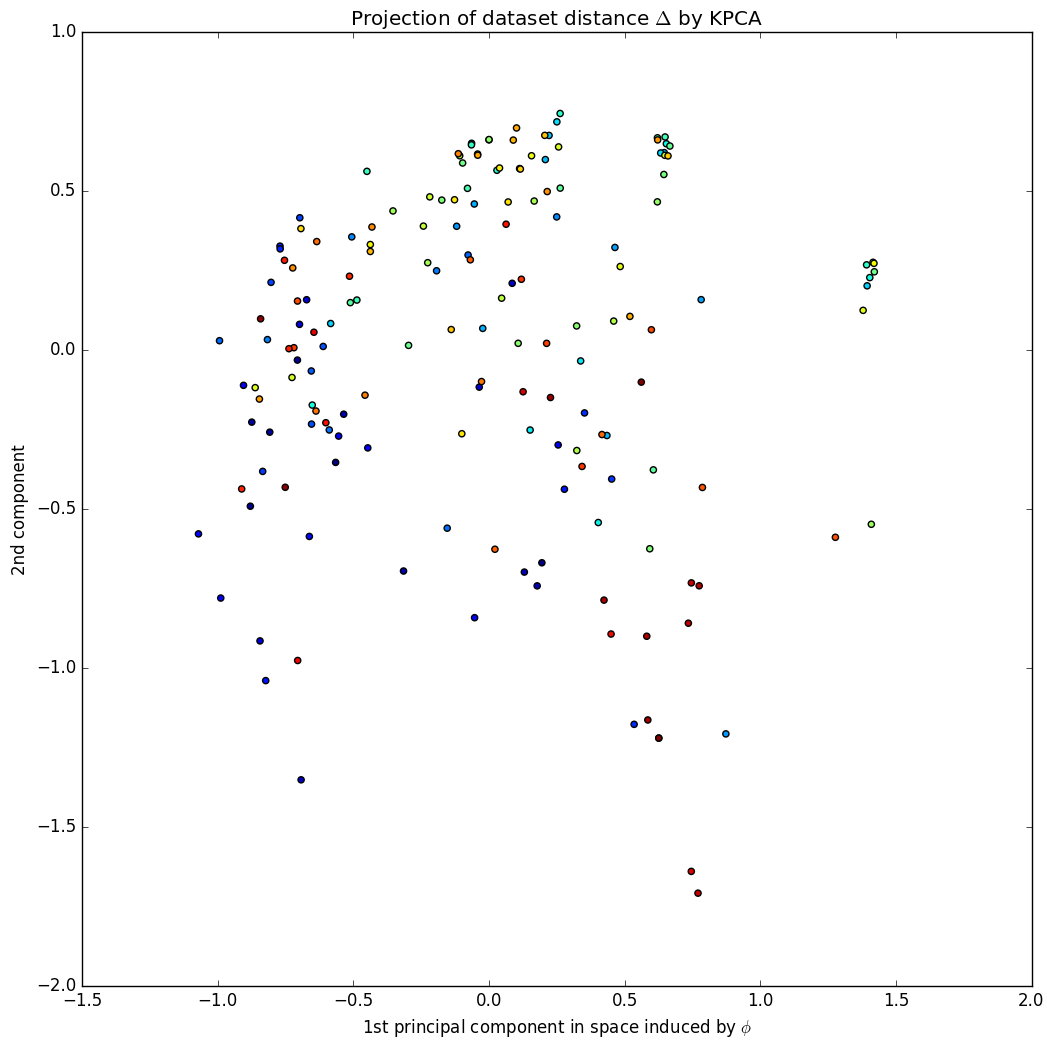
\includegraphics[width=14cm]{Images/kpcaDistance.png}
	\centering
	\caption{Projection of the training datasets using kernelized PCA and similarity based on the aggregation of global and attribute distance with the best result on the testing set.}	
	\label{fig:kpcaDistance}	
\end{figure}
 %file:///C:/Users/Jakub/OneDrive/Documents/Papers/RationalKernels.pdf
 